\documentclass{article}

\usepackage[french]{babel}
\usepackage[T1]{fontenc}
\usepackage{moreverb}       % verbatim with tab

\usepackage{wrapfig}
\usepackage{graphicx}
\usepackage{geometry}
\geometry{hmargin=2.5cm}
\usepackage{amsmath}
\usepackage{siunitx}

\usepackage{graphicx}
\usepackage{subcaption}
\usepackage{float}
\usepackage{hyperref}
\usepackage{setspace}
\usepackage{xcolor}
\usepackage{pdfpages}
\usepackage{enumitem}
\usepackage{lscape}

% https://tug.org/FontCatalogue/libertinusserif/
%\usepackage{libertinus}
%\usepackage[T1]{fontenc}

\usepackage{libertine} % Police Linux Libertine en sérif, Linux Biolinum en sans-sérif.

\usepackage[libertine]{newtxmath} % Math avec la police Libertine
%\addtokomafont{disposition}{\normalfont\sffamily} % Police des titres (ajouter \normalfont pour enlever le bold)
%\addtokomafont{paragraph}{\bfseries} % Titre des paragraphes en gras
%\addtokomafont{subsubsection}{\bfseries} % Titre des subsubsections en gras
%\usepackage[scaled=.8]{beramono} % Police monospace

\usepackage{fancyhdr}       % en-têtes
\usepackage{lastpage}       % numéro de dernière page

\title{Développement d'un codec audio AAC : optimisation de l'algorithme MDCT pour une architecture ARM}
\date{2020 -- 2021}
\author{Laura Binacchi}

\pagestyle{fancy}
\renewcommand\headrulewidth{1pt}
\fancyhead[L]{Laura Binacchi}
\fancyhead[C]{Développement d'un codec audio AAC}
\fancyhead[R]{2021 -- 2022}

\AtBeginDocument{
    \def\labelitemi{\textbullet}    % Redéfinition des puces dans les itemize
    \renewcommand{\times}{\text{×}} % Remplacer le gros «X» par un plus beau
    %\interfootnotelinepenalty=10000
}

\begin{document}
    \pagenumbering{gobble}
    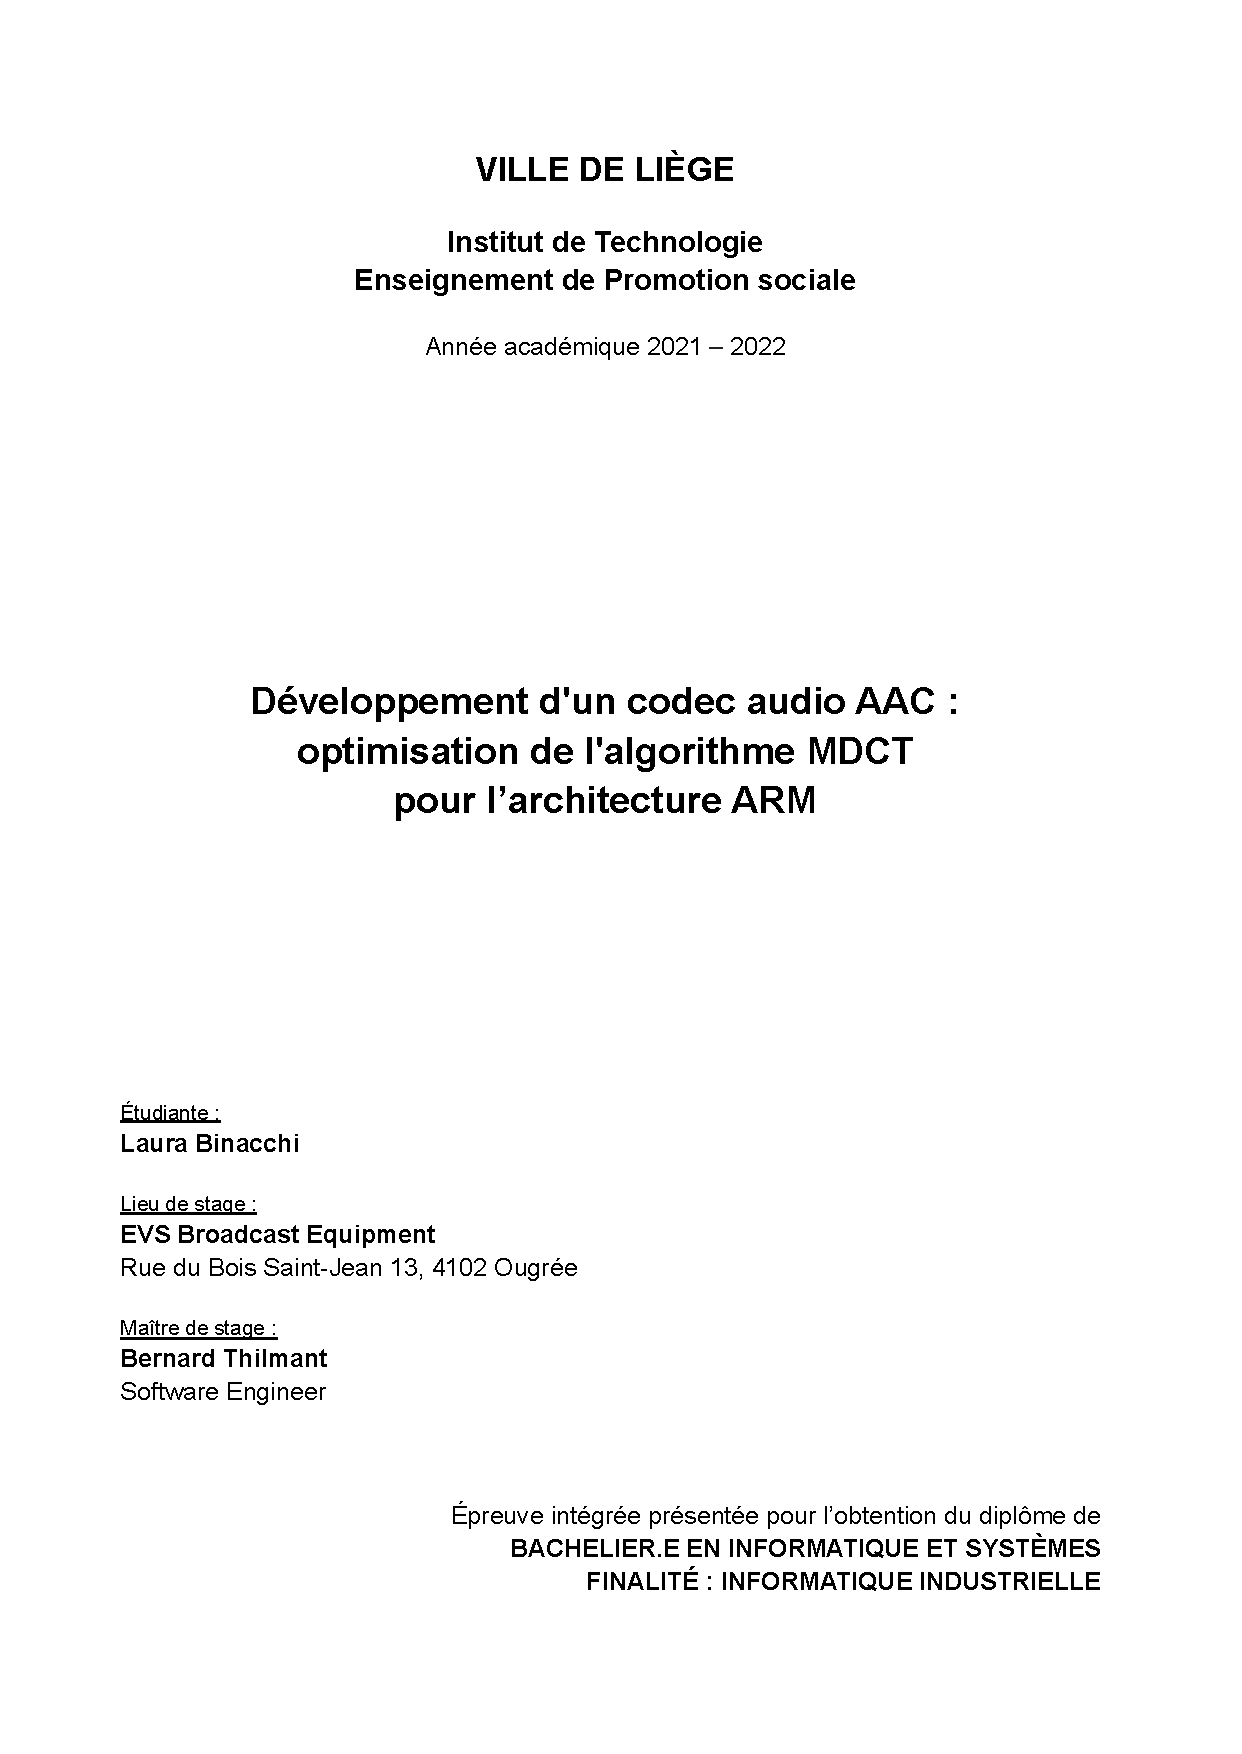
\includepdf[pages={1}]{pdg}
    \newpage
    \tableofcontents
    \newpage
    \pagenumbering{arabic}

    \section*{Remerciements}
    \paragraph{}

    \section*{Introduction}
    \addcontentsline{toc}{section}{\protect\numberline{}Introduction}

    % Contexte du projet : serveur XT (XT VIA qui succède à ...) et passage d'une architecture Intel à une architecture ARM
    % Travail qui s'inscrit dans la continuité d'un travail théorique préalable
    % Optimisations possibles et choix de l'algorithme MDCT (mais on pourrait aussi faire la même chose pour le bloc quantization, etc.)
    % Optimisations du bloc MDCT mises en place : passage d'une arithmétique floating à fixed point et utilisation des fonctions SIMD qui offrent une meilleur capacité de calcul
    % Limite de l'optimisation : limite de temps (temps du stage) plutôt que gain de performance par rapport à ce qui est déjà en prod

    \paragraph{}
    Développement d'une solution de software embarqué sur processeur ARM pour encodage audio AAC optimisé aux applications d'EVS :
    \begin{itemize}
        \item Prise de connaissance de l'encodage AAC et de l'environnement EVS qui utilise ce type de format ;
        \item Prise de connaissance des résultats des optimisations possibles du modèle psycho-acoustique développé par EVS ;
        \item Développement du code en C ou Assembler pour l'encodage AAC sur plateforme ARM ;
        \item Test du système et documentation de son implémentation.s possibles du modèle psycho-acoustique développé par EVS ;
        \item Développement du code en C ou Assembler pour l'encodage AAC sur plateforme ARM ;
        \item Test du système et documentation de son implémentation.
    \end{itemize}

    \paragraph{}
    %Mon travail s'inscrit dans la continuité de celui de Wafaa Heddari, stagiaire qui m'a précédée au sein du département hardware-firmware d'EVS pour y travailler sur le codec AAC. Après une étude du codec AAC et des différents blocs qui le composent, son mémoire dégage des pistes d'amélioration des performances du codec AAC : like Removal of block switching, Fast MDCT, and Optimized TNS. And then test their implementation on C Code to compare the compilation speed between the original Codec and the optimized one\cite{Wafaa}.

    %L'amélioration des performances est nécessaire par la qualité grandissante des données audio et video -> de plus en plus grandes, et le besoin de maintenir plusieurs flux en tant réel dans le broadcast



    \section{EVS Broadcast Equipment}
    \subsection{L'entreprise en quelques infos}




    \subsection{Le serveur XT}
    \paragraph{}
    EVS développe et commercialise de nombreux produits allant des serveurs de production aux interfaces permettant d'exploiter des données audio-visuelles ou de monitorer des systèmes de production\cite{EVS:products}. Le serveur de production live XT est un des produits emblématiques d'EVS. Il permet de stocker de grandes quantités de données audio-visuelles et d'y accéder en temps réel afin de répondre aux besoins de la production en live. Par exemple, la remote LSM (\emph{Live Slow Motion} permet d'accéder aux contenus des serveurs XT afin de créer les ralentis pour lesquels EVS est célèbre dans le monde.

    \begin{figure}[H]
        \centering
        \begin{subfigure}[b]{0.4\linewidth}
            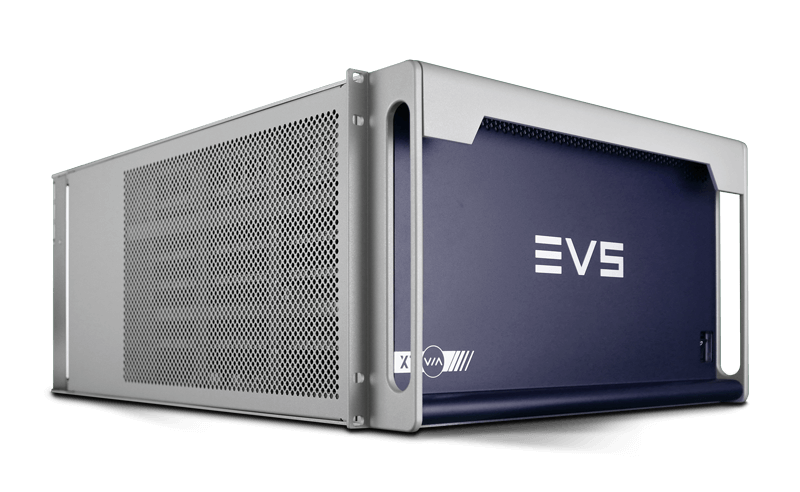
\includegraphics[width=\linewidth]{./images/XT-VIA.png}
        \end{subfigure}
        \begin{subfigure}[b]{0.4\linewidth}
            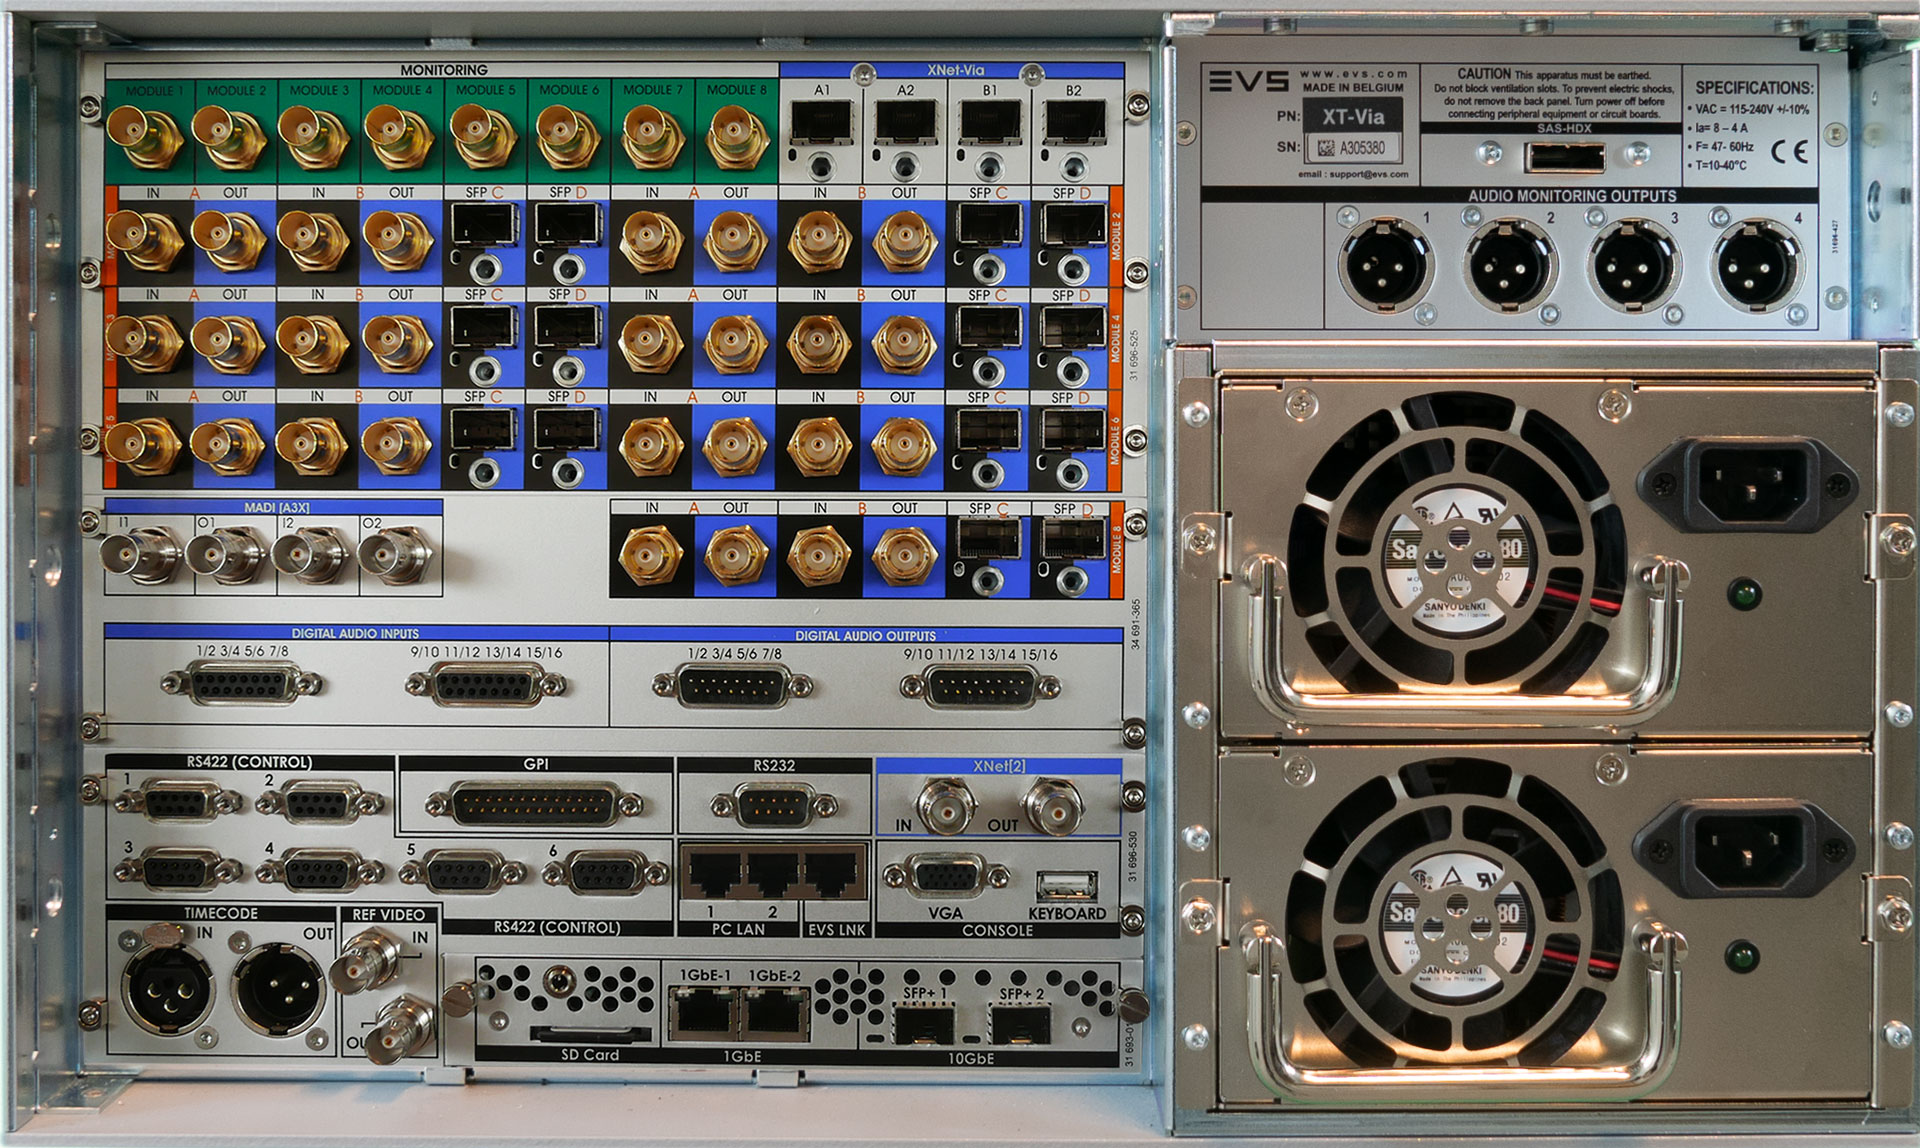
\includegraphics[width=\linewidth]{./images/XT-VIA-ar.jpg}
        \end{subfigure}
        \caption{Vues avant et arrière (en configuration IP) de l'XT-VIA}
    \end{figure}

%    \paragraph{}
%    Le serveur XT a connu plusieurs versions : XT, XT2, XT2+, XT3 et enfin l'XT-VIA. L'XT-VIA, la plus récente version du serveur XT, en quelques chiffres clés\cite{EVS:XT} :
%    \begin{itemize}
%        \item offre un espace de stockage de 18 à 54 TB, soit plus de 130h d'enregistrement en UHD-4k;
%        \item supporte de nombreux formats d'encodage : UHD-4K (XAVC-Intra et DNxHR), HD/FHD (XAVC-I, AVC-I, DNxHD et ProRes), PROXY (MJPEG et H264);
%        \item 
%    \end{itemize}
    
    % C'est pour cette dernière version, la plus récente de l'XT, que le codec AAC est développé. 

%    \paragraph{}
%    Afin de répondre aux exigences de la production live, en particulier d'événements sportifs, l'XT-VIA offre un espace de stockage de 18TB
%    \paragraph{}
%    En quelques chiffres clés

    \section{L'encodage audionumérique : généralités}
    \subsection{Le son}
    % onde acoustique -> 

    % - son audible = vibration entre 20 et 20kHz

    % le signal, analogique (continu) ou discret, peut avoir une représentation :
    % - temporelle
    % - fréquentielle
    % exemple de signaux périodiques (sinus, carré, etc) -> pp 6-7 + truc interactif

    % - spectre d'amplitude (utile) et spectre de phase (pas utile)

    % - toute fonction p(x, t) peut être exprimée par une somme de fonctions (co-)sinusoidales : formule pour les fonctions périodiques + transformée de Fourier pour les fonctions n'est pas périodique dans le temps

    \subsection{La numérisation d'un signal}
    % transformation de fourier :
    % https://www.claudegabriel.be/Math%C3%A9matiques%20appliqu%C3%A9es,%20chapitre%204.pdf -> p12 sur N pair / impair
    % à la base -> signaux périodique (faire bref)
    % -> ce qui nous intéresse : transformation pour signal non périodique discret -> DCT


    \section{Les codec audio}
    \subsection{Définition d'un codec}
    % avec et sans perte, etc
    \subsection{Historique des normes MPEG}


    %\paragraph{}
    %Le codec AAC est le dernier...
    %Le codec AAC a de nombreuses applications \cite{Wafaa}. Il est utilisé from low bitrate Internet audio to multichannel broadcasting services, thanks to its numerous working modes and configurations.

    %Le codec AAC est défin par le standard ISO/IEC 13818-7 : 




    \section{Le codec AAC}
    \subsection{Présentation générale}
    % présentation des différents blocs
    % \cite{wiki:AAC}

%In this thesis, we are going to study the different blocks of an AAC encoder based on the standard ISO/IEC 13818-7 such as the psychoacoustic model, Gain control, Transform block, Spectral processing, Quantization and Entropy coding. \cite{Wafaa}


    \subsection{Le bloc MDCT}
    % \begin{itemize}
    %     \item particularités par rapport à la FFT
    %     \item basée sur la DCT-IV
    %     \item niveaux de complexité (O...)
    % \end{itemize}


    \section{Développement de la MDCT}
    \subsection{Formule mathématique}



    \subsection{Fenêtre utilisée (autres paramètres ?)}
    % \begin{itemize}
    %     \item fenêtre de 1024
    %     \item pre-twiddle -> 256
    %     \item FFT
    %     \item post-twiddle -> 512
    % \end{itemize}
    \subsection{Algorithme de référence}
    % implémentation simple (en algo flottante), permet de valider les données des algos développés par la suite et d'en déterminer la précision


    \section{Optimisations algorithmiques}
    \subsection{Appel à un algorithme de FFT (nombres complexes)}
    % algo qui vient du code d'exemple dsprelated, basé sur la FFT
%    \url{https://infoscience.epfl.ch/record/59946}
%    \url{https://www.cis.rit.edu/class/simg716/Gauss_History_FFT.pdf}
%    \url{https://sci-hub.se/https://www.jstor.org/stable/29775194#}

    %jouer sur la symétrie pour ne calculer que la moitié

    % \subsection{Code DSP related}
    % Code qui se base sur une FFT avec opérations de pre et de post twiddle
    % Annexes : code de la MDCT, test et procédure d'installation de la librairie FFTW

    % au code de base, il faut aussi ajouter la fonction de fenêtre (MLT) qui n'était pas présente.


    \subsection{Réduction de la fenêtre d'entrée}
        % (pre et post processing/twiddles pour faire moins de FFT) -> réduction de la fenêtre de la FFT
    \subsection{Arithmétique fixed point}
    % \subsection{Arithmétique fixed point}
    % Le code de DSP related est en floating point -> passage en fixed point : opérations sur des entiers plus performantes + meilleure intégration (éviter le passage artificiel de l'entier au flottant et inversément)


    % à ce niveau, résultats pas intéressants car + d'opérations qu'en flottant et ARM a des fonctions d'algo flottante
    %     \paragraph{Rem} trivial en float (reprendre le code de dsp) mais pour l'implémentation en arithmétique entière, attention à mettre dans les bonnes ranges

    % \paragraph{Points d'attention}
    % \begin{itemize}
    %     \item les dépassements : 16 bits + 32 bits -> potentiellement 33 bits, 16*16 -> 32, etc. à voir en fonction des valeurs réelles
    %     \item alignement des tableaux (souvent c'est une contrainte imposée car permet facilement d'optimiser du code) : résolutions possibles en allouant dynamiquement les tableaux et en jouant avec une arithmétique de pointeur OU utilisation de posix mem align...
    % \end{itemize}

    % Attention à la manière d'écrire le code. Ici on n'a pas besoin de faire attention à ce que le compilateur puisse faire du inline (ex remplacer l'appel à z = add(a, d) par z = a+d pour économiser le call) car l'algo est déjà très optimisé -> pas d'optimisations de compilateur possible et en plus on a une grosse routine -> économiser un call n'est pas forcément intéressant.
    % Pas trop de C++ parce que faire un objet avec plein d'accessors, ce n'est pas très optimisé (on se retrouve avec un gros objet avec plein de variables). Derrière on fait de l'assembleur => il y a un trop grand écart. D'habitude les codesc audio sotn codés en C mais c'est aussi peut-être juste pour une raison historique.

    % Sur le format Qx.y :
    % https://www.pathpartnertech.com/representing-decimal-data-in-q-format/
    % https://www.allaboutcircuits.com/technical-articles/fixed-point-representation-the-q-format-and-addition-examples/
    % https://en.wikipedia.org/wiki/Q_(number_format)
    % et surtout https://web.archive.org/web/20171104111827/http://www.superkits.net/whitepapers/Fixed%20Point%20Representation%20%26%20Fractional%20Math.pdf

    % Intérêt de passer un integer: même si on ne gagne que 5\% de performance, on gagne du temps avant (les données qu'on reçoit sont en int16 -> pas de conversion vers le float après) et après (la quantification notament sera probablement plus rapide en integer)

    % Test de performance : il faut qu'à la fin l'implementation fixed point soit au moins aussi rapide que floating point



    \section{Optimisations à l'architecture ARM}
    \subsection{Spécificités de l'architecture ARMv8}
    \subsection{Utilisation de la FFT de la librairie Ne10}
    % FFT déjà optimisées pour Neon mais limitations sur ce qui entre et ce qui sort
    % \subsubsection{FFT de la librairie Ne10}
    % Le code de dsp related faisait appel à la librairie FFTW mais elle ne propose pas de FFT en fixed point => Ne10 qui propose une FFT fixed point optimisée pour ARM (avec ou sans instructions Neon)

    % Test de la librairie et des performances des différentes FFT : performances équivalentes en 32 bits (floating ou fixed) et deux fois plus rapides en 16 bits
    \subsection{Utilisation des fonctions Neon SIMD (intrinsic)}
    % \begin{itemize}
    %     \item voir la doc de neon \url{https://developer.arm.com/documentation/dht0002/a/Introducing-NEON/What-is-SIMD-/ARM-SIMD-instructions}
    %     \item voir comment faire ce qui doit être fait en fonction des instructions SIMD dispo : souvent il faut ranger correctement, splitter les registres correctement
    %     \item utilisation des instructions intrinsèques de GCC \url{https://fr.wikipedia.org/wiki/Fonction_intrins%C3%A8que}
    % \end{itemize}

    % Les opérations SIMD permettent de faire plusieurs opérations en uen fois où l'algo normal n'en fait qu'une à la fois. L'algo SIMD permet de faire plusieurs modifications à la fois -> il faut ranger les données de manière à pouvoir l'appliquer facilement (fonction fenêtre -> tri des données ? )

    % Plus les données sur lesquelles on travaille sont petites, plus on peut faire d'opérations en parallèle -> il faut voir si la perte de précision est ok. -> mettre une représentation graphique, c'est beaucoup plus simple à comprendre. D'où l'intérêt de passer à du 16 bits, plutôt que de rester en 32 bits et il faut absolument éviter le 64 bits (aucun intérêt).


    \section{Résultats}
    \subsection{Protocole de validation}
    %Validation aux différentes étapes des données : validation de la FFT, etc


    % \begin{itemize}
    %     \item sortie des données et générations de graphiques avec gnuplot
    %     \item résolution en fréquence pour une fenetre de 1024 samples pour un signal échantillonné à 48kHz : sur les graphiques $\frac{48000}{1024} = \SI{46.875}{\hertz}$ 1.3333... ms -> f = 1 / 1.33333 = 750 Hz OU res = fs / samples -> sur les graphiques on a des raies de fréquence de 750 Hz. Pour une fenêtre de 1024 = Hz
    % \end{itemize}
    % Graphiques sur sinusoide simple : augmenter la fréquence (i * qch pour déplacer la bande de fréquence), 

    %     Réaliser une fonction qui calcule la somme des cosinus (formule de wikipedia) pour chaque samples (pas du tout optimisée donc super lente). Pour la calcul en integer, on peut autoriser un manque de précision de max 1 LSB.


    % \begin{itemize}
    %     \item Voir les normes de test et règles d'acceptance des DCT et IDCT
    % \end{itemize}
    
    % \paragraph{}
    % Quand est-ce que la MDCT est assez optimisée ? Ici pas de critère de fin type 50 5 ou 2,5 \% plus rapide car pas de comparaison possible avec ce qui est actuellement en prod.

    % \paragraph{}
    % Pour les codecs c'est important de garder l'implémentation de référence mais à un moment on ne peut plus tester sur l'architecture intel. En pratique on utilise des pointeurs de fonction à déréférencer pour appeler l'implémentation voulue. En fonction du CPU ID, on sait quelles instructions on utilise. Au runtime, on choisit une ou l'autre implémentation en fonction de l'architecture, e.g. certains ARM n'ont pas les routines NEON



    \subsection{Gain en performance}
    % Comparaison avec un implémentation de référence plain c mais aussi à titre indicatif avec l'algorithme de référence car le plain c est déjà optimisé


    % L'impact de la window function : exemple avec un sinus : les composantes fréquentielles du sinus ressortent beaucoup mieux.

    \subsection{Perte de précision}
    % Comparaison avec l'algorithme de référence
    % Annexe : algo de référence, test de comparaison, résultats avec des données aléatoires et avec un sinus simple

    \newpage
    \section*{Conclusion}
    \addcontentsline{toc}{section}{\protect\numberline{}Conclusion}
    % Améliorations encore possible : faire les premières opérations de prétwiddling en Q15 8 par 8 avant de splitter, mêler les facteurs de la fenêtre aux facteurs de twiddling

    \bibliography{biblio} 
    \bibliographystyle{ieeetr.bst}
    \addcontentsline{toc}{section}{\protect\numberline{}Références}
    
\end{document}